\documentclass[10pt,a4paper]{article}	
\usepackage{amsmath}
\usepackage{amsfonts}
\usepackage{amssymb}
\usepackage{cite}												% 支持引用多篇文献
\usepackage{CJK}													% 支持中文
\usepackage{indentfirst}                 						% 首行缩进宏包
\usepackage{graphicx}											% 支持图片的插入
\usepackage{subfigure}											% 支持插入子图
\usepackage[colorlinks,citecolor = blue, linkcolor=blue,hyperindex,CJKbookmarks]{hyperref}				% 链接功能
\usepackage{fancyhdr}											% 添加页眉
\usepackage{array}												% 使用表格
\usepackage{multirow}

\newcommand{\PreserveBackslash}[1]{\let\temp=\\#1\let\\=\temp}	% 表格固定
\newcolumntype{C}[1]{>{\PreserveBackslash\centering}p{#1}}		% 宽度并且
%\newcolumntype{R}[1]{>{\PreserveBackslash\raggedleft}p{#1}} 		% 使用居中
\newcolumntype{L}[1]{>{\PreserveBackslash\raggedright}p{#1}}		% 排列方式
\graphicspath{{figs/}}                              				% 图片文件夹路径
\setlength{\parindent}{2em}										% 缩进距离为2个字符位置
\newcommand{\song}{\CJKfamily{song}}     						% 宋体
\newcommand{\hei}{\CJKfamily{hei}}       						% 黑体
\newcommand{\fs}{\CJKfamily{fang}}         						% 仿宋
\newcommand{\kai}{\CJKfamily{kai}}       						% 楷体
\newcommand{\li}{\CJKfamily{li}}         						% 隶书
\newcommand{\you}{\CJKfamily{you}}       						% 幼圆
\newcommand{\chuhao}{\fontsize{42pt}{\baselineskip}\selectfont}     % 字号设置
\newcommand{\xiaochuhao}{\fontsize{36pt}{\baselineskip}\selectfont} % 字号设置
\newcommand{\yichu}{\fontsize{32pt}{\baselineskip}\selectfont}      % 字号设置
\newcommand{\yihao}{\fontsize{28pt}{\baselineskip}\selectfont}      % 字号设置
\newcommand{\erhao}{\fontsize{21pt}{\baselineskip}\selectfont}      % 字号设置
\newcommand{\xiaoerhao}{\fontsize{18pt}{\baselineskip}\selectfont}  % 字号设置
\newcommand{\sanhao}{\fontsize{15.75pt}{\baselineskip}\selectfont}  % 字号设置
\newcommand{\sihao}{\fontsize{14pt}{\baselineskip}\selectfont}      % 字号设置
\newcommand{\xiaosihao}{\fontsize{12pt}{\baselineskip}\selectfont}  % 字号设置
\newcommand{\wuhao}{\fontsize{10.5pt}{\baselineskip}\selectfont}    % 字号设置
\newcommand{\xiaowuhao}{\fontsize{9pt}{\baselineskip}\selectfont}   % 字号设置
\newcommand{\liuhao}{\fontsize{7.875pt}{\baselineskip}\selectfont}  % 字号设置
\newcommand{\qihao}{\fontsize{5.25pt}{\baselineskip}\selectfont}    % 字号设置

\renewcommand{\baselinestretch}{1.1} %定义行间距


\begin{document}

\begin{CJK*}{UTF8}{song}

\renewcommand\contentsname{目录}

% 添加封面

%%% Local Variables:
%%% mode: latex
%%% TeX-master: t
%%% End:
\secretlevel{保密} \secretyear{2}

\ctitle{同济大学学位论文 \LaTeX{} 模板使用示例}

% 按照申请工学学位设计。如有其它需要,请修改相应文字。
\makeatletter
  \iftongji@doctor
    \cdegree{工学博士}
  \else
    \iftongji@master
      \cdegree{工学硕士}
    \fi
  \fi

\makeatother

\cdepartment{同济大学Linux用户组}

\cmajorfirst{Linux}

\cmajorsecond{Linux}

\cauthor{同济人}

\csupervisor{裴钢 教授}

% 如果没有副指导老师或者联合指导老师,把各自{}中内容留空即可。

\cassosupervisor{万钢 教授}

\ccosupervisor{三钢 教授}

% 日期自动生成,如果你要自己写就改这个cdate
%\cdate{\CJKdigits{\the\year}年\CJKnumber{\the\month}月}
\makeatletter
  \iftongji@doctor
    \edegree{Doctor of Philosophy}
  \else
    \iftongji@master
      \edegree{Master of Science}
    \fi
  \fi

\makeatother

\cfunds{(国家杰出青年基金 (No.123456789) 支持)}

\efunds{(Supported by the Natural Science Foundation of China for\\ Distinguished
         Young Scholars, Grant No.123456789)}

\etitle{A Simple Sample of Tongji Thesis\\ Using \tongjithesis{}}

\edepartment{TONGJILUG}

\emajorfirst{TONGJILUG}

\emajorsecond{TONGJILUG}

\eauthor{Tongji Ren}

\esupervisor{Prof. Gang Pei}

\eassosupervisor{Prof. Gang Wan}

% 这个日期也会自动生成,你要改么?
% \edate{May, 2009}

% 定义中英文摘要和关键字
\begin{cabstract}
  论文的摘要是对论文研究内容和成果的高度概括。摘要应对论文所研究的问题及其研究目
  的进行描述,对研究方法和过程进行简单介绍,对研究成果和所得结论进行概括。摘要应
  具有独立性和自明性,其内容应包含与论文全文同等量的主要信息。使读者即使不阅读全
  文,通过摘要就能了解论文的总体内容和主要成果。

  论文摘要的书写应力求精确、简明。切忌写成对论文书写内容进行提要的形式,尤其要避
  免“第 1 章……;第 2 章……;……”这种或类似的陈述方式。

  本文介绍同济大学论文模板 \tongjithesis{} 的使用方法。本模板符合学校的硕士、
  博士论文格式要求。

  本文的创新点主要有:
  \begin{itemize}
    \item 用例子来解释模板的使用方法;
    \item 用废话来填充无关紧要的部分;
    \item 一边学习摸索一边编写新代码。
  \end{itemize}

  关键词是为了文献标引工作、用以表示全文主要内容信息的单词或术语。关键词不超过 5
  个,每个关键词中间用分号分隔。(模板作者注:关键词分隔符不用考虑,模板会自动处
  理。英文关键词同理。)
\end{cabstract}

\ckeywords{\TeX, \LaTeX, CJK, 模板, 论文}

\begin{eabstract}
   An abstract of a dissertation is a summary and extraction of research work
   and contributions. Included in an abstract should be description of research
   topic and research objective, brief introduction to methodology and research
   process, and summarization of conclusion and contributions of the
   research. An abstract should be characterized by independence and clarity and
   carry identical information with the dissertation. It should be such that the
   general idea and major contributions of the dissertation are conveyed without
   reading the dissertation.

   An abstract should be concise and to the point. It is a misunderstanding to
   make an abstract an outline of the dissertation and words ``the first
   chapter'', ``the second chapter'' and the like should be avoided in the
   abstract.

   Key words are terms used in a dissertation for indexing, reflecting core
   information of the dissertation. An abstract may contain a maximum of 5 key
   words, with semi-colons used in between to separate one another.
\end{eabstract}

\ekeywords{\TeX, \LaTeX, CJK, template, thesis}



%%%%%%%%%%%%%%%%%%%%%%%%%%%%%%%%%%%%%%%%%%%%%%%%%%%%%%%%
%%                          目录                      %%
%%%%%%%%%%%%%%%%%%%%%%%%%%%%%%%%%%%%%%%%%%%%%%%%%%%%%%%%
\newpage
\pagestyle{fancy} 
\lhead{}
\chead{\small{目录}}
\rhead{}
\tableofcontents
\pagenumbering{Roman}

%添加符号标记
%
\newpage
\pagestyle{fancy} 
\lhead{}
\chead{\small{符号}}
\rhead{}

大写加粗的字母代表矩阵,比如说$\mathbf{X}$。默认情况下,向量都是指列向量,并且用小写的粗斜体表示。比如$\mathbf{X}=[\boldsymbol{x_{1}},\boldsymbol{x_{2}},\cdots,\boldsymbol{x_{m}}]$是一个包含$m$个列向量$\boldsymbol{x_{i}},i=1,\cdots,m$
的矩阵$\mathbf{X}$。向量$\boldsymbol{x_{j}}$的第$i$个元素表示为$[\boldsymbol{x_{j}}]_i$。对于没有下标的向量$\boldsymbol{x}$也是表示列向量$\boldsymbol{x}=[x_1,\cdots,x_n]^T$。对于矩阵$\mathbf{X}$第$i$行第$j$列的元素可以表示为$[\mathbf{X}]_{i,j}$。文中所有符号见下表\ref{notation}。



\begin{table}[!htp]
\caption{符号定义表}
\label{notation}
\center
\begin{tabular}{C{2.5cm}L{7.5cm}}
\hline
符号 				& 	含义		\\ 
\hline
$\mathbb{N}$			&	自然数集和\\
$\mathbb{R}$ 		&	实数集合 	\\
$\mathcal{X}$ 		&  	输入空间 	\\
$\mathcal{Y}$ 		&	输出空间	\\
$\mathcal{D}$ 		&	对输入空间进行判定后获得的集合	\\
$\mathcal{H}	$		&	特征空间 	\\
$f$					&	判定函数$f:\mathcal{X}\rightarrow\mathcal{D}$ 	\\
$q$					&	分类原则$q:\mathcal{X}\rightarrow\mathcal{Y}$	\\
$\langle\boldsymbol{x},\boldsymbol{x'}\rangle$	&	$\boldsymbol{x}$和$\boldsymbol{x'}$的点乘	\\
$k(\boldsymbol{x},\boldsymbol{x'})$	&	核函数	\\
$\boldsymbol{\mu}$	&	均值向量	\\
$\mathbf{S}$			&	离散度矩阵$\mathbf{S}=\sum_{i=1}^{m} (\boldsymbol{x_i}-\mu)(\boldsymbol{x_i}-\mu)^T$\\
$\mathcal{T_X}$		&	未被标记的训练集$\mathcal{T_X}=\{x_1,\cdots,x_m\}$\\
$\mathcal{T_XY}$		&	标记的训练集$\mathcal{T_XY}=\{(x_1,y_1),\cdots,(x_m,y_m)\}$	\\
$m$					&	训练样本的数目\\
$n$					&	输入空间的维度\\
$\mathbf{E}$			&	单位矩阵\\
\hline
\end{tabular}
\end{table}


%%%%%%%%%%%%%%%%%%%%%%%%%%%%%%%%%%%%%%%%%%%%%%%%%%%%%%%%
%%                          正文                      %%
%%%%%%%%%%%%%%%%%%%%%%%%%%%%%%%%%%%%%%%%%%%%%%%%%%%%%%%%
\newpage

%============================++题目和作者++================================
\pagestyle{fancy} 
\lhead{}
\chead{\small{同济大学课程报告}}
\rhead{}
\title{PCA系列方法的研究报告}					% 题目
\author{王菲\thanks{学院:电信学院;\;专业:计算机技术;\;学号:1433378;\;Email:wangfei\_tongjics@126.com}}									% 作者
%============================++++++++++++=================================
\date{}                                             				% 显示作者,不显示日期
\maketitle                                          				% 生成标题
\pagenumbering{arabic}


\section{引言}
自从1901年卡尔·皮尔逊发明主成分分析法\cite{1}(Principal components analysis,PCA)以后,PCA就成立一个强有力的工具。主成分分析法是一种分析、简化数据集的技术,常用于减少数据集的维数,同时保持数据集中的对方差贡献最大的特征。由于PCA具有最大化方差、最小化冗余、最小化损失等优良特性,它可以广泛地应用在多源融合、数据降维、模式识别以及分析数据相关性等方面。如已经发表的人脸识别中PCA方法的推广\cite{3}和基于L2,1范数的PCA维数约简算法\cite{4},PCA在其中起了提取主元和维数简约预处理的重要作用。虽然以后出现了大量其他方法,如LDA和一些非线性的算法,如SVM,神经网络等算法,并广泛地应用在各个领域,如机器学习、图像检索、模式识别和人工智能等方面。但PCA作为一种基本的线性方法,其地位是其他方法所无法比拟的。


主成分分析法是将多个变量综合成少数变量的一种多元统计方法,可以有效地来处理变量间的线性关系,为解决多指标的综合评价提供了一种很好的手段。但现实中特征间的关系往往是非线性的,所以线性PCA的方法就无法正确的体现样本特征。而随着核方法的引入,使得核主成分分析方法\cite{5}(KPCA)算法能够很好的处理非线性数据集。它首先选取核函数简爱嗯数据集隐式的映射到高维空间,实现线性数据向线性数据的转换,然后在高维空间进行主成分分析。


近年来,由于计算机技术的高速发展,各种数据量以指数级的速度增加,各种大规模数据广泛地出现在各个计算机领域。但是目前计算机硬件的发展仍然满足不了数据处理的要求。比如在人脸识别中,图像的尺寸为128×128,而整个图片集又有3000张,那么在图像分类中把图片当成一个列的大距阵将是16384×3000,这是非常大的矩阵,计算复杂度高,其中最费时的部分就是在最后一步分解矩阵\cite{2}来求的特征值和特征向量。所以另一种基于贪心算法的快速主成分分析方法就产生了。该算法在保持了与KPCA相同的处理效果的同时,降低了时间复杂度,增加了算法稳定性,减少了内存使用率,从而使得计算时间大大缩短。
\newpage

\section{PCA的发展史}
主元分析法(PCA)是最简单的以特征量分析多元统计分布的方法。其结果可以理解为对原数据中的方差做出解释:哪一个方向上的数据值对方差的影响最大?换而言之,PCA提供了一种降低数据维度的有效办法;如果分析者在原数据中除掉最小的特征值所对应的成分,那么所得的低维度数据必定是最优化的(也即,这样降低维度必定是失去讯息最少的方法)。在其发展过程中,主成分分析法(PCA)首先借助核方法克服其无法处理非线性问题的弱点,生成了核主元分析法(KPCA),紧接着又利用贪心算法使其计算时间大大缩减,生成了贪心核主元分析法(GKPCA)。下面将详细介绍这三个阶段的PCA算法。

\subsection{主元分析法(PCA)}
\subsubsection{问题描述}
假定有m个n维的训练样本$\mathcal{T_X}=\{x_1,\cdots,x_m\}$,如何能够用一个n维的向量$\boldsymbol{x_0}$来最好的代表这m个样本,或者更确切的说,我们希望这个代表向量$\boldsymbol{x_0}$与各个样本$\boldsymbol{x_k},k=1,\cdots,m$的距离的平方之和越小越好。定义平方误差准则函数$\mathcal{J}_0(\boldsymbol{x_0})$如下,
\begin{equation}
\mathcal{J}_0(\boldsymbol{x_0})=\sum_{k=1}^{m}\Vert\boldsymbol{x_0}-\boldsymbol{x_k}\Vert
\end{equation}
很容易想到,这个问题的答案就是$\boldsymbol{x_0}=\boldsymbol{\mu}$,其中$\boldsymbol{\mu}$是样本的均值,即
\begin{equation}
\boldsymbol{\mu}=\sum_{k=1}^{m}\boldsymbol{x_k}
\end{equation}
样本均值是样本数据集的零维表达。它非常简单,但缺点是并不能反映出样本之间的不同。通过把全部样本向通过样本均值的一条直线作投影,我们能够得到代表全部样本的一个一维向量。让$\boldsymbol{e}$表示这条通过骆样本均值的直线上的单位向量,那么这条执行的方程可以表示为
\begin{equation}
\label{direction}
\boldsymbol{x}=\boldsymbol{\mu}+a\boldsymbol{e}
\end{equation}
其中$a\in\mathbb{R}$,表示直线上某个点离开$\boldsymbol{\mu}$的距离。如果我们用$\boldsymbol{\mu}+a_k\boldsymbol{e}$来代表$\boldsymbol{x_k}$,那么最小化平方误差准则函数为
\begin{eqnarray}
\label{minsquerr}
\mathcal{J}_1(a_1,\cdots,a_m,\boldsymbol{e})\nonumber
&=&\sum_{k=1}^{m}\Vert(\boldsymbol{\mu}+a_k\boldsymbol{e})-\boldsymbol{x_k}\Vert^2\\
&=&\sum_{k=1}^{m}a_k^2\Vert\boldsymbol{e}\Vert^2-
2\sum_{k=1}^{m}a_k\boldsymbol{e}^T(\boldsymbol{x_k}-\boldsymbol{\mu})+
\sum_{k=1}^{m}\Vert\boldsymbol{x_k}-\boldsymbol{\mu}\Vert^2 
\end{eqnarray}
由于$\Vert\boldsymbol{e}\Vert=1$,通过对$a_k$求偏导,并且令结果为0,我们得到
\begin{equation}
\label{opitialdirection}
a_k=\boldsymbol{e}^T(\boldsymbol{x_k}-\boldsymbol{\mu})
\end{equation}
从几何上说,这个结果告诉我们只要把向量$\boldsymbol{x_k}$向通过样本均值的直线作垂直投影就能够得到最小方差结果。

这就引起一个更有意义的问题,即,如何找到直线$\boldsymbol{e}$的最优方向。将公式\ref{opitialdirection}得到的$a_k$带入到公式\ref{minsquerr}中,我们可以看到
\begin{eqnarray}
\label{mseans}
\mathcal{J}_1{\boldsymbol{e}}
&=&\sum_{k=1}^{m}a_k^2-2\sum_{k=1}^{m}a_k^2+
\sum_{k=1}^{m}\Vert\boldsymbol{x_k}-\boldsymbol{\mu}\Vert^2 \nonumber \\
&=&-\sum_{k=1}^{m}\boldsymbol{e}^T(\boldsymbol{x_k}-\boldsymbol{\mu})(\boldsymbol{x_k}-\boldsymbol{\mu})^T\boldsymbol{e} \nonumber \\
&=&-\boldsymbol{e}^T\mathbf{S}\boldsymbol{e}
+\sum_{k=1}^{m}\Vert\boldsymbol{x_k}-\boldsymbol{\mu}\Vert^2 
\end{eqnarray}
在公式\ref{mseans}中,显然使$\mathcal{J}_1$最小的那个向量$\boldsymbol{e}$,能够使$\boldsymbol{e}^T\mathbf{S}\boldsymbol{e}$最大。我们使用拉格朗日乘子法来最大化$\boldsymbol{e}^T\mathbf{S}\boldsymbol{e}$,约束条件为等式$\Vert\boldsymbol{e}\Vert=1$,求解得
\begin{equation}
\label{pacans}
\mathbf{S}\boldsymbol{e}=\lambda\boldsymbol{e}
\end{equation}
所以很自然地得出结论,为了最大化$\boldsymbol{e}^T\mathbf{S}\boldsymbol{e}$,我们选取散布矩阵$\mathbf{S}$最大的特征值对应的那个特征向量作为投影直线$\boldsymbol{e}$的方向。


这一结论可以立刻从一维空间的映射推广到$d(d\leqslant{}n)$维空间的映射。将公式\ref{direction}重写为
\begin{equation}
\label{mulpc}
\boldsymbol{x}=\boldsymbol{\mu}+\sum_{i=1}^{d}a_i\boldsymbol{e_i}
\end{equation}
不难证明,新的平方误差准则函数
\begin{equation}
\label{mulms}
\mathcal{J}_{d}=\sum_{k=1}^{m}\Vert(\boldsymbol{\mu}+\sum_{i=1}^{d}a_i\boldsymbol{e_i})-\boldsymbol{x_k}\Vert^2   
\end{equation}
在向量$\boldsymbol{e_1},\cdots,\boldsymbol{e_{d}}$分别为散布矩阵的$d$个最大特征值所对应的特征向量,取得最小值。因为散布矩阵是实对称矩阵,因此这些特征向量都是相互正交的。这些特征向量构成了代表任一向量$\boldsymbol{x}$的基向量。公式\ref{mulpc}中的系数$a_i$对应于基$\boldsymbol{e_i}$的系数,被称作主成分。从几何上说,样本点$\boldsymbol{x_1}.\cdots,\boldsymbol{x_m}$在n维空间形成了一个n维椭球形状的云团。那么散布矩阵的特征向量就是这个云团的主轴。主成分分析通过提取云团散布最大的那些方向的方法,达到了对特征空间进行降维的目的。

\subsubsection{算法描述}
根据上面的描述,很容易写出如下PCA算法。
\begin{table}[!htp]
\label{notation}
\center
\begin{tabular}{|L{0.9\textwidth}|}
\hline
\textit{算法1}:主元分析法(PCA) \\
\hline
\end{tabular}
\end{table}
\begin{enumerate}
\item 计算训练数据$\mathcal{T_X}=\{x_1,\cdots,x_m\}$的离散矩阵$\mathbf{S}$[协方差矩阵的m-1倍]
\item 计算离散矩阵的特征值$\mathbf{\Lambda}=diag(\lambda_1,\cdots,\lambda_d),\lambda_1\geqslant\cdots\geqslant\lambda_d$和特征向量$\mathbf{U}=[\boldsymbol{\mu_1},\cdots,\boldsymbol{\mu_{d}}]$
\item 将d个特征向量进行斯密特正交化$\mathbf{E}=[\boldsymbol{e_1},\cdots,\boldsymbol{e_{d}}]$
\item 根据公式\ref{opitialdirection}和公式\ref{mulpc}可以计算出经过映射后在主轴上的点
\end{enumerate}


\subsubsection{程序实现}
用matlab编程,随机生成样本点,并获得如下图\ref{fig:pca}所示的结果:
\begin{figure}[!htbp]
	\centering
	\caption{PCA算法}  
		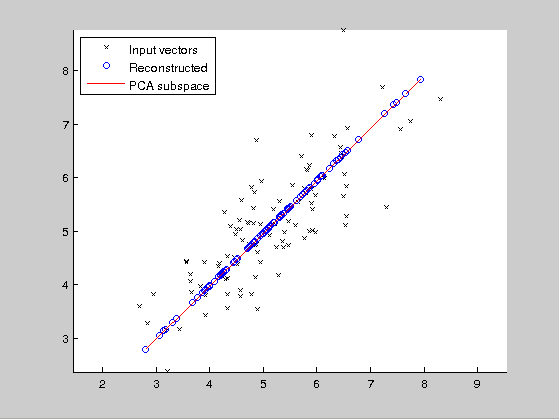
\includegraphics[scale=0.55]{figs/pca.png}
    	\label{fig:pca}
\end{figure}
图中黑色的叉代表输入的训练样本点,蓝色的圈代表样本点投影到主轴上的点,而红色的直线代表训练样本集的主轴方向。很明显,主轴的方向明显的表现了训练样本点的数据特征。


\subsection{核主元分析法(KPCA)}
\subsubsection{核方法}
核方法(kernel methods,KMs)是一类模式识别的算法。其目的是找出并学习一组数据中的相互的关系。用途较广的核方法有支持向量机(SVM)、高斯过程等。


核方法是解决非线性模式分析问题的一种有效途径,其核心思想是:首先,通过某种非线性映射将原始数据映射到合适的高维特征空间;然后,利用通用的线性学习器在这个新的空间中分析和处理模式。相对于使用通用非线性学习器直接在原始数据上进行分析的范式,核方法有明显的优势:首先,通用非线性学习器不便反应具体应用问题的特性,而核方法的非线性映射由于面向具体应用问题设计而便于集成问题相关的先验知识。再者,线性学习器相对于非线性学习器有更好的过拟合控制,从而可以更好地保证泛化性能。还有,很重要的一点是,核方法还是实现高效计算的途径,它能利用核函数将非线性映射隐含在线性学习器中进行同步计算,使得计算复杂度与高维特征空间的维数无关。


核方法中比较关键的就是核函数的选择,它通过一个非线性变换$\phi$将原始空间映射到一个新的特征空间,即
\begin{equation}
\mathbf{X}=[\boldsymbol{x_1},\cdots,\boldsymbol{x_m}] \qquad
\Longrightarrow \qquad
\phi(\mathbf{X})=[\phi(\boldsymbol{x_1}),\cdots,\phi(\boldsymbol{x_m})]
\end{equation}
根据Hilbert-Schmidt定理,只要给定的变换$\phi$满足Mercy定理\cite{6},就可用于构建核函数。采用不同的核函数可以获得不同的核分类器,它们的性能也各不相同,在特定的数据集上,某些核函数将表现出更优的性能。常用的核函数有:
\begin{itemize}
\item 线性核	$k(\boldsymbol{x},\boldsymbol{x'})=\langle \boldsymbol{x},\boldsymbol{x'} \rangle$
\item 多项式核	$k(\boldsymbol{x},\boldsymbol{x'})=(\langle \boldsymbol{x},\boldsymbol{x'} \rangle+k)^n$
\item 径向基核	$k(\boldsymbol{x},\boldsymbol{x'})=\frac{exp(-\langle \boldsymbol{x},\boldsymbol{x'} \rangle^2)}{\sigma^2}$
\item Sigmoid核	$k(\boldsymbol{x},\boldsymbol{x'})=\tanh(v\langle \boldsymbol{x},\boldsymbol{x'} \rangle+k)$
\end{itemize}
在某些情况下,用简单的核函数可以形成复合核,从而实现更复杂的非线性映射。

\subsubsection{问题描述}
假定有训练集$\mathbf{X}=[x_1,\cdots,x_m]\in \mathbb{R}^{n*m}$,我们需要根据最小平方误差的准则来重新构建该训练集或者提取其主要特征,我们的目标是寻找一个线性正交化的映射
\begin{equation}
\label{map}
\boldsymbol{y}=\mathbf{W}^T\boldsymbol{x}+\boldsymbol{b}
\end{equation}
能够将输入$\boldsymbol{x} \in \mathbb{R}^n$变换为低维输出$\boldsymbol{y} \in \mathbb{R}^d,d<n$。其中矩阵$\mathbf{W} \in \mathbb{R}^{n*d}$和向量$\boldsymbol{b} \in  \mathbb{R}^d$是该映射的参数。我们用$\tilde{\mathbf{X}}=[\tilde{x_1},\cdots,\tilde{x_m}]\in \mathbb{R}^{n*m}$来表示经过$\mathbf{Y}=[y_1,\cdots,y_m]\in \mathbb{R}^{d*m}$重构后的向量矩阵。由公式\ref{map}可以得到$\tilde{\boldsymbol{x}}$的表达式
\begin{equation}
\label{inverse}
\tilde{\boldsymbol{x}}=\mathbf{W}(\boldsymbol{y}-\boldsymbol{b})
\end{equation}
那么平方误差就可以定义为
\begin{equation}
\varepsilon_{MS}=\frac{1}{m}\sum_{i=1}^{m}\Vert \boldsymbol{x_i}-\tilde{\boldsymbol{x_i}} \Vert^2
\end{equation}
易知该公式和公式\ref{mulms}是等价的。所以到此可以按照上面求解训练数据集的离散度矩阵$\mathbf{S}$和均值向量$\boldsymbol{\mu}$,然后求解其d个最大的特征值$\mathbf{\Lambda}=diag(\lambda_1,\cdots,\lambda_d),\lambda_1\geqslant\cdots\geqslant\lambda_d$和对应的特征向量$\mathbf{W}=[\boldsymbol{w_1},\cdots,\boldsymbol{w_{d}}]$。$\mathbf{W}$是$\varepsilon_{MS}$取得最小值时所对应的变换矩阵。而最优误差向量$\boldsymbol{b}$等于$-\mathbf{W}^T\boldsymbol{\mu}$.所以公式\ref{inverse}可以进一步化简为
\begin{equation}
\tilde{\boldsymbol{x}}=\mathbf{W}\boldsymbol{y}+\boldsymbol{\mu}
\end{equation}

核主元分析法是采用了核方法的,所以主元分析法的整个过程是可以用向量的点乘来表示的。假定$\hat{\mathbf{X}}=\mathbf{X}-\mathbf{X}\mathbf{M}$表示中心化了的训练数据,其中$\mathbf{M} \in \mathbb{R}^{m*m}$是一个所有元素都是$\dfrac{1}{m}$的矩阵。所以中心化的训练样本数据的点乘为
\begin{eqnarray}
\label{centering}
\hat{\mathbf{X}}^T\hat{\mathbf{X}}
&=&(\mathbf{X}-\mathbf{X}\mathbf{M})^T(\mathbf{X}-\mathbf{X}\mathbf{M})\nonumber\\
&=&\mathbf{X}^T\mathbf{X}-\mathbf{M}^T\mathbf{X}^T\mathbf{X}
-\mathbf{X}^T\mathbf{X}\mathbf{M}+\mathbf{M}^T\mathbf{X}^T\mathbf{X}\mathbf{M}
\end{eqnarray}
其特征值及其特征向量为$\mathbf{\Lambda}$和$\mathbf{U}$.有下面等式
\begin{equation}
\hat{\mathbf{X}}^T\hat{\mathbf{X}}\mathbf{U}=\mathbf{U}\Lambda
\end{equation}
其中$\mathbf{U}=[\boldsymbol{u_1},\cdots,\boldsymbol{u_d}] \in \mathbb{R}^{m*d}$是点乘矩阵$\hat{\mathbf{X}}^T\hat{\mathbf{X}}d$个特征向量正交化后的矩阵,而另一个矩阵$\Lambda=diag(\lambda_1,\cdots,\lambda_d) \in \mathbb{R}^{d*d},\lambda_1\geqslant\cdots\geqslant\lambda_d$是由d个成递减顺序的特征值构成的对角矩阵。
经过化简得
\begin{eqnarray}
(\hat{\mathbf{X}}\hat{\mathbf{X}}^T)(\hat{\mathbf{X}}\mathbf{U})
=(\hat{\mathbf{X}}\mathbf{U})\Lambda\\
(\hat{\mathbf{X}}\mathbf{U})^T(\hat{\mathbf{X}}\mathbf{U})=\mathbf{U}^T\mathbf{U}\Lambda=\Lambda
\end{eqnarray}
那么离散矩阵$\hat{\mathbf{X}}\hat{\mathbf{X}}^T$的正交化后的特征向量$\mathbf{V}=[\boldsymbol{v_1},\cdots,\boldsymbol{v_d}] \in \mathbb{R}^{n*d}$可以表示为
\begin{equation}
\label{scatter}
\mathbf{V}=\hat{\mathbf{X}}\mathbf{U}\Lambda^{-\frac{1}{2}}=\hat{\mathbf{X}}\mathbf{B}
\end{equation}
其中$\Lambda^{-\frac{1}{2}}=diag(\dfrac{1}{\sqrt{\lambda_1}},\cdots,\dfrac{1}{\sqrt{\lambda_d}})$是对角矩阵,$\mathbf{B}=\mathbf{U}\Lambda^{-\frac{1}{2}}$
最后公式\ref{map}可以化简为
\begin{eqnarray}
\label{mapping}
\boldsymbol{y}&=&\mathbf{V}^T(\boldsymbol{x}-\boldsymbol{\mu})\nonumber\\
&=&(\mathbf{B}-\mathbf{M}\mathbf{B})^T\mathbf{X}^T\boldsymbol{x}-
\mathbf{B}^T\mathbf{X}^T\mathbf{X}\boldsymbol{m}
+\mathbf{B}^T\mathbf{M}^T\mathbf{X}^T\mathbf{X}\boldsymbol{m}
\end{eqnarray}
很明显,训练数据的中心化\ref{centering},特征向量的分解\ref{scatter}以及训练数据的线性映射\ref{mapping}都是只需要点乘。

\subsubsection{算法描述}
根据上面的描述,很容易写出如下KPCA算法。
\begin{table}[!htp]
\label{notation}
\center
\begin{tabular}{|L{0.9\textwidth}|}
\hline
\textit{算法2}:核主元分析法(KPCA) \\
\hline
\end{tabular}
\end{table}
\begin{enumerate}
\item 计算训练数据$\mathcal{T_X}=\{x_1,\cdots,x_m\}$的核矩阵$K \in \mathbb{R}^{m*m},[K]_{i,j}=k(\boldsymbol{x_i},\boldsymbol{x_j}),i,j=1,\cdots,m$
\item 计算中心化后的核矩阵$\tilde{K}$
\begin{equation}
\tilde{\mathbf{K}}=\mathbf{K}-\mathbf{M}^T\mathbf{K}-\mathbf{K}\mathbf{M}
+\mathbf{M}^T\mathbf{K}\mathbf{M}
\end{equation}
\item 求解中心化后的矩阵的特征值$\Lambda \in \mathbb{R}^{m*m}$和特征向量$\mathbf{U} \in \mathbb{R}^{m*m}$
\item 取d个最大的特征值$\Lambda=diag(\lambda_1,\cdots,\lambda_d) \in \mathbb{R}^{d*d},\lambda_1\geqslant\cdots\geqslant\lambda_d$对应的特征向量$\mathbf{U}=[\boldsymbol{u_1},\cdots,\boldsymbol{u_d}]$。并计算$\mathbf{B}=\mathbf{U}\Lambda^{-\frac{1}{2}}$
\item 根据公式\ref{mapping}计算训练样本点的映射
\end{enumerate}


\subsubsection{程序实现}
用matlab编程,随机生成三类样本点,采用径向基核函数进行主元分析,获得如下图\ref{kpca}所示的结果:
\begin{figure}[!htbp]
  \begin{minipage}[t]{0.48\linewidth}
    \centering
    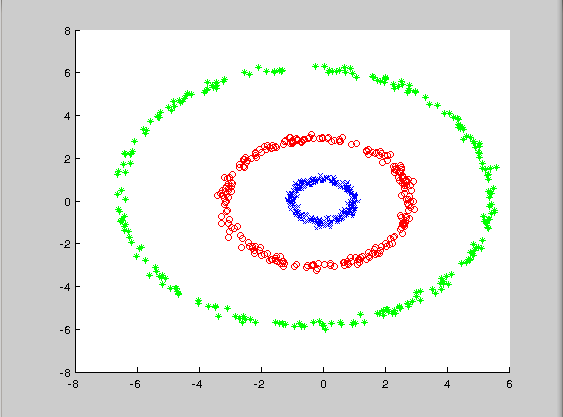
\includegraphics[width=\textwidth]{figs/kpca_pre.png}
    \caption{生成随机数据\label{kpca_pre}}
  \end{minipage}
  \hfill
  \begin{minipage}[t]{0.48\linewidth}
    \centering
    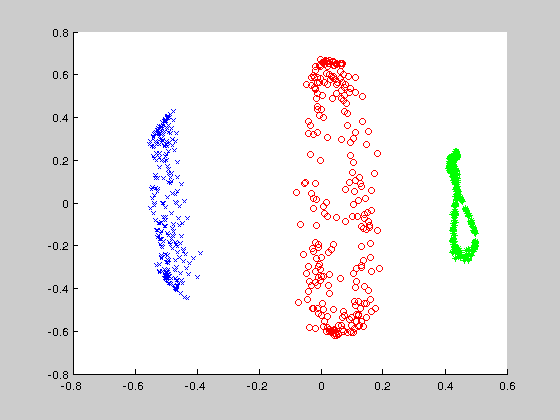
\includegraphics[width=\textwidth]{figs/kpca_deal.png}
    \caption{径向基核映射\label{kpca_deal}}
  \end{minipage}
  \label{kpca}
\end{figure}
由数据可知,KPCA使得原本线性不可分的数据变得线性可分了。


核主成分分析(KPCA)是将原空间的数据通过非线性变换映射到特征空间中,在特
征空间中进行主成分分析,不需要知道$\phi$的具体形式,只需在原空间中进行点积运算即可。
只要选取适当的核,就会得到比PCA较明显的降维效果,避免了PCA中因主成分贡献率过于分散而
影响评价效果;同时KPcA能有效地处理变量间的非线性关系。而对于不同的核函数具有什么不同的性质,
它们各自适用于什么样的情况这方面是值得进一步挖掘。



\subsection{贪婪核主元分析法(GKPCA)}
\subsubsection{问题描述}
从上面核主元分析法(KPCA)算法中可以看出,KPCA能够处理非线性问题,其一般的表达式为
\begin{equation}
f{x}=\sum_{i=1}^m \alpha_i\langle \Phi(x),\Phi(x_i) \rangle+b
=\sum_{i=1}^m \alpha_i k(x,x_i) +b
\end{equation}
但是该算法仍然有两个问题。
\begin{enumerate}
\item 训练阶段中,核矩阵的规模将会极大影响算法性能。\\
随着训练样本数目的增加,核矩阵的规模成二次增加。这样对于大量的训练数据集,核矩阵的存储就成一个问题。另一方面,对核矩阵的求特征值和特征向量也将会使得算法变慢。
\item 在判定阶段,求解出的参数矩阵中非零系数太多也会使得算法性能大大降低。\\
虽然大部分学习算法像支持向量机模型产生稀疏结果,但是非零系数的数目还是太多,特别是当训练样本太多或者训练样本中出现大量重复样本时。此外,像KPCA和KFDA不是一定产生系数结果。
\end{enumerate}
而贪婪核主元分析法(GKPCA)的提出就是为了优化上面提出的两个问题。


假定样本训练集$\mathcal{T}=[x_1,\cdots,x_m]$代表特征空间$\mathcal{H}$。我们想要选择训练样本的子集$\mathcal{S} \subset \mathcal{T}$来代表训练样本$\mathcal{T}$,当然$\mathcal{S}$和$\mathcal{T}$的线性跨度是要一致的。再假定$\mathcal{I}={1,\cdots,m}$代表训练集$\mathcal{T}$的索引集,而$\mathcal{J}={1,\cdots,l}$代表挑选的训练子集$\mathcal{S}$的索引集。而通过训练子集$\mathcal{S}$可以构造新的训练样本$\tilde{\mathcal{T}}=[\tilde{x_1},\cdots,\tilde{x_m}]$。
\begin{equation}
\tilde{f}{x}=\sum_{j \in \mathcal{J}} \beta_j\langle \Phi(x_j),\Phi(x) \rangle+\theta
=\sum_{j \in \mathcal{J}} \beta_j k(x_j,x) +\theta
\end{equation}
换而言之,对于原始的训练样本的估计$\tilde{\boldsymbol{x_i}}$都可以用挑选的训练子集来表示,即
\begin{equation}
\tilde{\boldsymbol{x_i}}=\sum_{j \in \mathcal{J}} \boldsymbol{x_i}[\mathbf{\beta_i}]_j, \quad \forall_i \in \mathcal{I}
\end{equation}
其中$\mathcal{J} \subset \mathcal{I}$有l个挑选的训练样本,$\beta_i \in \mathbb{R}^l,i \in \mathcal{I}$是线性组合的系数。那么平方误差就可以表示为
\begin{equation}
\label{gpcame}
\varepsilon_{MS}(\boldsymbol{T}|\boldsymbol{J})=
\frac{1}{m}\sum_{i \in \mathcal{I}}\Vert \boldsymbol{x_i}-\tilde{\boldsymbol{x_i}} \Vert^2
=\frac{1}{m}\sum_{i \in \mathcal{I}}\Vert \boldsymbol{x_i}-\sum_{j \in \mathcal{J}} \boldsymbol{x_j}[\mathbf{\beta_i}]_j \Vert^2
\end{equation}
当我们选定训练样本子集$\mathcal{J}$后就可以确定$\beta_i$。
\begin{equation}
\beta_i=\arg\min_{\beta \in \mathbb{R}^l}
=\Vert \boldsymbol{x_i}-\sum_{j \in \mathcal{J}} \boldsymbol{x_j}[\mathbf{\beta_i}]_j \Vert^2
=(\mathbf{K_s})^{-1}\boldsymbol{k}_s(x_i), \quad \forall_i \in \mathbf{I}
\end{equation}
其中$\mathbf{K}_s \in \mathbb{R}^{l*l}$是挑选样本的核矩阵。向量$\mathbf{k_s}(x_i)=[k(x_{j1},x_i),\cdots,k(x_{jl},x_i)]^T \in \mathbb{R}^l$是挑选的训练矩阵$\mathcal{S}$和$x_i$经过核方法处理后的向量。将上式公式代入平方误差公式\ref{gpcame},得到
\begin{equation}
\varepsilon_{MS}(\boldsymbol{T}|\boldsymbol{J})=
\frac{1}{m}\sum_{i \in \mathcal{I}}(k(x_i,x_i)-2\mathbf{K_s}\boldsymbol{k_s}(x_i)+
\langle \boldsymbol{k_s}(x_i),\mathbf{K_s}\boldsymbol{k_s}(x_i) \rangle)
\end{equation}
最终问题就变成从训练样本$\mathcal{T}$挑选l个训练样本构成集合$\mathcal{J}$,使得$\varepsilon_{MS}(\boldsymbol{T}|\boldsymbol{J})$最小,即
\begin{equation}
\mathcal{J^*}=\arg\min_{\mathcal{J} \in \mathcal{I}}\varepsilon_{MS}(\boldsymbol{T}|\boldsymbol{J})
\end{equation}

\subsubsection{算法描述}
根据上面的描述,很容易获得简单的贪心核主元分析(GKPCA)算法。
\begin{table}[!htp]
\label{notation}
\center
\begin{tabular}{|L{0.9\textwidth}|}
\hline
\textit{算法3}:简单贪婪核主元分析法(simple-GKPCA) \\
\hline
\end{tabular}
\end{table}
\begin{enumerate}
\item 初始化\\
$\mathcal{J}^{0}=\{\varnothing\}$
\item 执行循环\\
For t = 1 to l:
\begin{enumerate}
 \item[(a)] 
 $
 j_t \in \arg\min_{j \in \mathcal{I}\setminus\mathcal{J}^{t-1}}
 \varepsilon_{MS}(\boldsymbol{T}|\boldsymbol{J}^{(t-1)} \cup \{j\})
 $
 \item[(b)] 
 $
 \mathcal{J}^{(t)}=\mathcal{J}^{(t-1)} \cup \{ j_t\}
 $
\end{enumerate} 
\end{enumerate}
显而易见,该算法是对从m个训练样本中找l个代表样本所有$C_m^l$种可能的遍历。在Step(b)中需要$\mathcal{O}(m^2)$。所以整个算法的复杂度达到了$\mathcal{O}(lm^2)$。因为对$\boldsymbol{x_i}$的估计误差一定小于误差出错的最大值,所以存在下面的不等式对上述算法进行优化
\begin{equation}
\varepsilon_{MS}(\boldsymbol{T}|\boldsymbol{J})
=\frac{1}{m}\sum_{i \in \mathcal{I}}\Vert \boldsymbol{x_i}-\tilde{\boldsymbol{x_i}} \Vert^2
\leqslant \frac{1}{m}(m-l)\max_{j \in \mathcal{I} \setminus \mathcal{J}} \Vert \boldsymbol{x_j}-\tilde{\boldsymbol{x_j}} \Vert^2
\end{equation}
\begin{table}[!htp]
\label{notation}
\center
\begin{tabular}{|L{0.9\textwidth}|}
\hline
\textit{算法4}:贪婪核主元分析法(GKPCA)\cite{9} \\
\hline
\end{tabular}
\end{table}
\begin{enumerate}
\item 寻找贪心列\\
计算中心化核矩阵$\tilde{\mathcal{K}}$每个列向量的范数,选择其中范数最大的n列排列起来构成$\tilde{\mathcal{K}}$的一个m×n的子矩阵$\tilde{\mathcal{K}}_n$
\item  构造低维卷数据\cite{7}\cite{8}矩阵\\
对$\tilde{\mathcal{K}}_n$做QR分解来得到一个矩阵Q,Q的列向量组成了一个构成$\tilde{\mathcal{K}}_n$列向量的一个正交基。然后构造卷数据低维矩阵$\mathbf{A}=(\mathbf{C}\mathbf{Q})^T$.
\item 低维矩阵分解\\
设$\mathbf{A}$的SVD分解为
\begin{equation}
\mathbf{A}=\sum_{i=1}^m \lambda_i \mathbf{V}_i(\boldsymbol{u_i}^T)
\end{equation}
\end{enumerate}
从上面的算法中可以看出三步的时间复杂度分别为$\mathcal{O}(m),\mathcal{O}(n^2m),\mathcal{O}(n^2m)$。所以总的时间复杂度为$\mathcal{O}(m^2)$。所以算法复杂度比一般算法低一阶。


\subsubsection{程序实现}
用matlab编程,随机生成一组250样本的训练集,分别采用KPCA和GKPCA方法对样本进行处理,获得如下图\ref{greedkpca}所示的结果:
\begin{figure}[!htbp]
  \begin{minipage}[t]{0.48\linewidth}
    \centering
    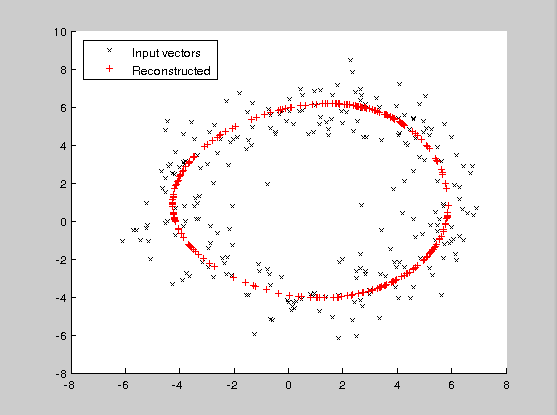
\includegraphics[width=\textwidth]{figs/kpca.png}
    \caption{kpca方法\label{kpca}}
  \end{minipage}
  \hfill
  \begin{minipage}[t]{0.48\linewidth}
    \centering
    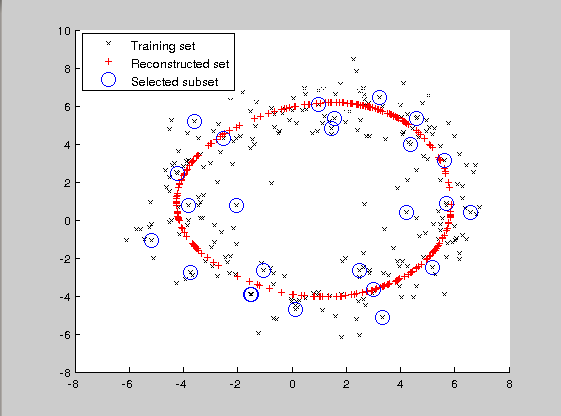
\includegraphics[width=\textwidth]{figs/gkpca.png}
    \caption{gkpca方法\label{kpca}}
  \end{minipage}
  \label{greedkpca}
\end{figure}
由图可知,GKPCA获得的处理效果基本跟KPCA无差别。但这两种方法所花费的时间如下表\ref{compare}所示。
\begin{table}[!htp]
\label{compare}
\center
\begin{tabular}{C{0.3\textwidth}C{0.3\textwidth}C{0.3\textwidth}}
\hline
样本数	&	KPCA	/s	&	GKPCA/s\\
\hline
100		&	0.3989	&	0.2850\\
200		&	0.5254	&	0.3633\\
300		&	0.8159	&	0.4593\\
400		&	1.0912	&	0.4608\\
500		&	1.4069	&	0.5615\\
600		&	1.7395	&	0.6350\\
\hline
\end{tabular}
\end{table}
由上表可知随着样本数的递增,两个算法解决问题所花的时间也在随着增加,但是在过程中KPCA所花的时间明显比GKPCA花的多。

\newpage
\section{PCA的应用}
\subsection{主元分析法PCA}
PCA的应用方向很多,主要应用于多源融合、数据降维、分析数据互相关性以及模式识别中,下面就遥感图像融合和采用TPCA(二次PCA)做图像边缘提取做简要的说明。
\subsubsection{遥感图像融合}
为了将多频谱段拍摄的遥感图像以及高分辨率的图像融合在一起从而获得包含多个谱段信息的高分辨率图像,可以采取的办法是将多谱段每个图像看成列向量,并将其组成矩阵A,对矩阵A进行PCA主成分分析,可以得到一系列主元,由于段谱段图像之间均经过配准且具有较高的相关度,他们之间只是存在细微的区别,我们的目的是保留这些细微的区别,因此将第一个主元替换为高分辨率的图像,对所有主元进行重建,所得到的图像即为融合后图像。其流程图如下图\ref{yaogan}所示
\begin{figure}[!htbp]
	\centering
	\caption{遥感图像融合流程}  
		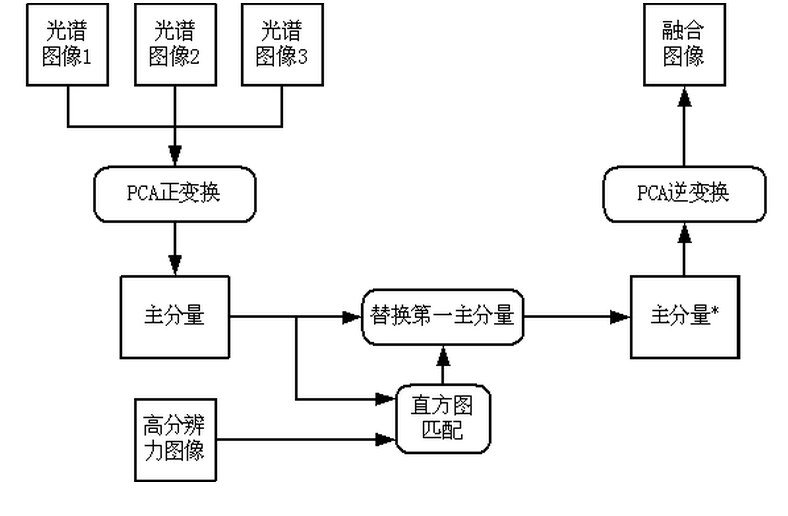
\includegraphics[scale=0.55]{figs/yaogan.png}
    	\label{fig:yaogan}
\end{figure}

\subsection{TPCA图像分割}
由于PCA在数据集聚上具有方向性,为了提高类内聚合度, 需选择能将尽量多的相似数据聚在一起的投影方向, 这就说明PCA总是从数据集中找相似的数据子集, 且每个子集内的类内离散度要最小, 即数据要相似, 其反映在图像上就是灰度值要一致。当用部分主分量来近似表示数据集时, 图像中的大块灰度平滑区域就能被抽取出来, 其中与较大特征值对应的特征向量就是由灰度平滑区域的数据构成的。   


另外PCA技术在处理单幅图像时, 在垂直方向上存在方向性。由于PCA是将列看成一类, 为了使类内散布度最小, 在重建图像时, 其找到的最佳投影方向会将同一列中的数据向灰度均值方向拉平。在垂直边缘处, 由于两边的灰度产生突变, 因此为了保证类内散度最小, 重建部分会在垂直边缘处产生模糊, 使该
列上的所有像素的灰度相互靠拢,如下图\ref{tpca}所示。
\begin{figure}[!htbp]
	\centering
	\caption{原图与重建图}  
		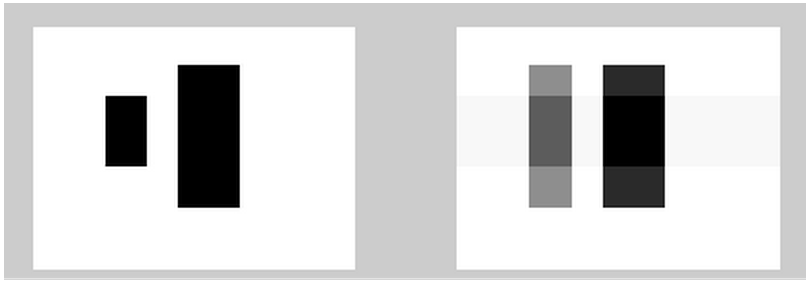
\includegraphics[scale=0.55]{figs/tpca.png}
    	\label{fig:tpca}
\end{figure}


黑块的上下两端都产生了模糊现象,这表明经过PCA处理后, 边缘处的像素灰度产生了变化, 像素由白色和黑色变成灰色, 也就是灰度值变变化, 像素由白色和黑色变成灰色, 也就是灰度值变因此利用PCA的这种方向特性, 就可以通过检测这种变化来检测边缘。根据以上特点,在水平和垂直方向均做PCA(TPCA),这样两方向的边缘均提取出来。其与其他几种算子的对比如下图\ref{compare4}所示
\begin{figure}[!htbp]
	\centering
	\caption{TPCA流程图以及各边缘提取算法对比}  
		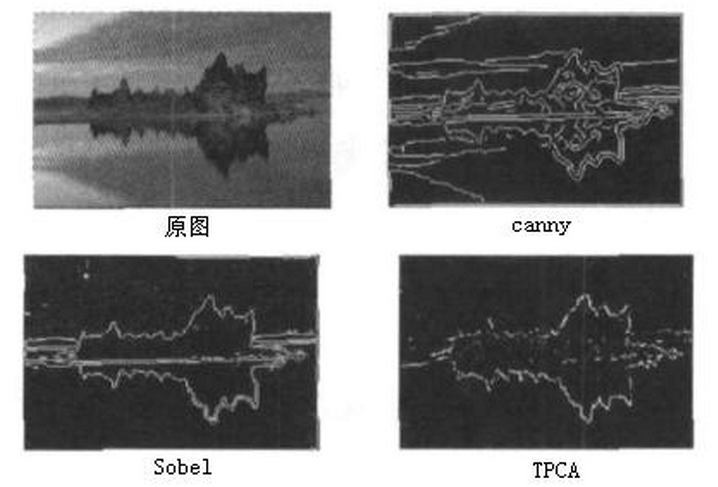
\includegraphics[scale=0.55]{figs/compare4.png}
    	\label{fig:compare4}
\end{figure}


\subsection{核主元分析法KPCA}
\subsubsection{人脸识别}
采用国际上常用的ORL的人脸数据库,该数据库包括40个人的400幅图像,每个人的脸像为10幅,
具有不同的光照、表情和视点。采用双线性插值法将原图像处理为32×32以减少计算量,
而不会影响识别率。如图\ref{face}所示。
\begin{figure}[!htbp]
	\centering
	\caption{ 部分人脸图像}  
		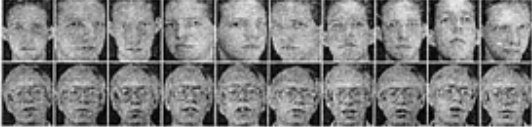
\includegraphics[scale=0.55]{figs/face.png}
    	\label{fig:face}
\end{figure}
任取200幅图像作训练,200幅作测试。即每人5幅图像作训练样本,另外的5幅作测试样本。
分别采用KPCA和PcA进行人脸特征提取,为计算简单,这里取多项式核函数。在获得有效的特征后,
利用支持向量机(SVM)设计分类器。其中,对于KPCA得到的人脸特征,
直接设计线性SVM分类器;而对于PCA得到的人脸特征,
采用文献\cite{10}中的SVM分类器设计方法。实验结果如下表\ref{kpcaface}。
\begin{table}[!htp]
\label{kpcaface}
\center
\begin{tabular}{C{0.6\textwidth}C{0.4\textwidth}}
\hline
方法		&	错误率	\\
\hline
KPCA d=2		&	2.61	\\
KPCA d=3		&	2.52	\\
KPCA d=4		&	1.72	\\
KPCA d=5		&	1.78	\\
PCA			&	4.85	\\
\hline
\end{tabular}
\end{table}
通过实验数据可知。由于KPCA考虑了图像像索之间的
非线性关系,从而使识别的正确率与传统的PCA有了明显的
提高。当核函数阶次d=4时,错误率达到最低。

\subsection{贪婪核主元分析法GKPCA}
贪婪核主元分析法(GKPCA)是对KPCA算法的一个优化,二者的目的都是相同的,不同的地方在于算法的复杂度有很大的差异。这也就导致到GKPCA更适合于处理有大量训练样本或者核矩阵规模比较大的情况。特别是下面的两种情况:
\begin{enumerate}
\item 训练阶段,核矩阵的规模很大。\\
随着训练样本数目的增加,核矩阵的规模成二次增加。这样对于大量的训练数据集,核矩阵的存储就成一个问题。另一方面,对核矩阵的求特征值和特征向量也将会使得算法变慢。
\item 判定阶段,求解出的参数矩阵中非零系数太多\\
虽然大部分学习算法像支持向量机模型产生稀疏结果,但是非零系数的数目还是太多,特别是当训练样本太多或者训练样本中出现大量重复样本时。此外,像KPCA和KFDA不是一定产生系数结果。
\end{enumerate}
对于上面提出的情况,只要满足任意一点,就可以用GKPCA来提高降低算法的复杂度,提高算法解决问题的效率。



\newpage
\section{研究意义及挑战}
\subsection{研究意义}
本文主要提出了三个PCA系列的算法,分别是PCA,KPCA,GKPCA。
通过比对PCA和KPCA之间的关系,我们可以得到下面的结论
\begin{itemize}
\item PCA仍然不失为一种好分析方法. 数据呈非线性流形分布, 或者说是各指标呈非线性关系式时, 对于线性分析分析方法来说可能效果不是特别好, 但同时应该注意的是它也是一种统计分析方法. 实际经济指标中都存在线性相关性 (信息冗余 ), 这是符合统计规律的, 完全不相关的经济数据是极其少见, 也就是说要求的数据只要大致呈线性分布, 而且有PCA计算简单, 无需先念知识、无需参数设置等优点.
\item PCA与线性核KPCA不完全一样. 对于有n个指标的m个数据样本, PCA计算协方差阵为n*n维矩阵, 它可以提取的主成分为n.而KPCA是从核矩阵出发计算的, 最大可以提取的主成分为m.为满足在特征空间中的样本均值为零, 还要对核矩阵K进行特殊处理, 这也是导致与线性核与原样本内积的不一致的原因.
\item KPAC核函数与核参数难于选择, 不同的核函数及其核参数对排序结果影响很大, 甚至出现完全相反的结果. KPC 的这个特点严重的影响了它的实用价值.PCA的协方差矩阵的特征向量对应于各经济指标在主成分的比重, 从而能用原经济指标去解释主成分. 而KPCA的是基于是核矩阵的特征向量, 与原指标没有对应关系, 从而核主成分解释困难. 其次KPCA将指标投影到高维特征空间后, 而其实际的数据又是在原空间处理的, 其数值在原空间中是否均有排序意义也值得进一步研究.
\item 数据的归一化处理对输出结果有一定的影响, 在应用时, 为了消除量纲,应该对数据进行归一化处理.
\end{itemize}
通过对比KPCA和GKPCA之间的关系,我们也可以得到下面的结论
\begin{itemize}
\item 当矩阵规模比较大时,算法在保持分解质量即特征值不变的前提下,速度至少比标准的KPCA算法快了一倍多。.
\item 当所构建的低维空间的维度减小时,尽管此时运算速度会加快,但是与标准算法相比会出现偏差,当运算精度要求不高,运算时间比较珍贵时,可以采取此法。 
\end{itemize}


\subsection{研究挑战}
在研究的过程中,发现有些问题到目前为止还需要进一步探究。
\begin{itemize}
\item 核函数的选取\\
在KPCA算法中,我们发现对于相同的训练样本集,选取不同的核函数会产生不同的结果。虽说核函数的选取只要满足Mercy定理,但是对于不同的情况,选取合适的核函数依以此来产生好的效果,显然对于不同核函数的性质还要进一步挖掘
\item 求矩阵特征值和特征向量这个问题能否进一步优化\\
研究到GKPCA才发现,我们要做的工作是对KPCA算法进行优化。之歌可以转变成求解特征值和特征向量的问题。
\end{itemize}

%\newpage		
%\section{致谢}
%衷心感谢两位老师上课的深入浅出的讲解,是我们对课程知识有了透彻的了解。虽然对黄老师那全英文的授课方式有点感冒,但是知道老师也是为了我们好,所以后来也在积极努力的去融入这样的氛围中,并且享受这个过程。授课的内容也是偏向于具体的知识。而另外一位王老师却专注于启发我们的思维。我想这两样对于我们今后的科研都是非常有帮助的。具体知识是基础,发散的思维则是创新的来源。所以非常感谢两位老师一学期以来的教导。
%
%除了上课的老师外,我还要感谢我的导师何良华。虽然他没帮我做啥,但是当我有任何学习上的问题时,他都能给出方向上的指引。
\newpage
\bibliographystyle{unsrt}										% 按引用的先后顺序排列,比较次序为作者,年度和标题
\bibliography{ref/mybib}												% 引用文件数据库在bib.bib文件中

\clearpage     
\end{CJK*}
\end{document}
